\documentclass[a4paper]{jacow}


\usepackage{graphicx}       % Extended support for \includegraphics
\usepackage{mathptmx}       % Mathematical PostScript fonts
\usepackage{amsmath}        % General mathematical symbols
\usepackage{url}            % \url command for decent line breaks in urls
\usepackage{enumitem}       % For more control over list parameters.

\hyphenpenalty 500 % Tone down hyphenation

\begin{document}
\title{NEW FEATURES AND MEASUREMENTS USING THE UPGRADED TRANSVERSE MULTIBUNCH FEEDBACK AT DIAMOND}

\author{G.~Rehm, M.G.~Abbott, A.F.D.~Morgan,
    Diamond Light Source, Oxfordshire, UK}

\maketitle

\begin{abstract}

A Transverse Multi-Bunch Feedback has been used in the Diamond Storage Ring for the stabilization of instabilities since 2007. Following a recent upgrade of the FPGA code and EPICS layer, a set of new features is now available to support operation and machine development: Firstly, a bunch by bunch choice of feedback filter allows for better stabilization of a single high charge bunch in a hybrid fill pattern. Secondly, complex grow-damp experiments are now possible using a sequencer of internal states allowing precise measurements of the damping rates on a mode by mode basis. Thirdly, a phase locked loop excitation and detection has been implemented to allow both extremely fast (kHz update rates) and extremely precise tracking of the betatron tune frequencies. Finally, short FIR filters on the ADC input and DAC output enable a fine tuning of the impulse response to provide maximum bunch to bunch isolation, as for instance required for efficient bunch cleaning.

\end{abstract}


\section{Introduction}

At Diamond we stabilise transverse oscillations of the bunches with two FPGA
based Transverse Multi-Bunch Feedback (TMBF) processors, one operating
horizontally, one vertically.  Each processor is a Libera Bunch-by-Bunch from
Instrumentation Technologies \cite{libera}, packaged as a 1U unit containing 4
14-bit ADCs running at 125\,MHz, a Virtex-II Pro FPGA clocked at 125\,MHz, a
14-bit DAC running at 500\,MHz, and an embedded Single Board Computer (SBC) ARM
microprocessor running Linux to provide the control system.

The system was delivered as a basic development platform with interfacing
software on the Linux board and a layer of FPGA code for interfacing to the
external signals and the processor board.  The initial implementation of the
Transverse Multi-Bunch Feedback (TMBF) processor was done at Diamond
\cite{early-tmbf} based on work at the ESRF \cite{esrf}.  The Diamond
implementation consists of FPGA code together with an EPICS driver running on
the embedded processor board.

Diamond has been using transverse multibunch feedback since 2007
\cite{performance}.  The firmware and software have continued to develop and include
functionality beyond the pure feedback action required for suppression of
multibunch instabilities, most importantly a numerically controlled oscillator (NCO), which can be used to excite bunches and detect their oscillation in phase with the excitation.

The developments described in this paper
provide support for more detailed measurements, finer control, and more complex
experiments.  In particular, the following major functionality has been added in a recent upgrade of FPGA and EPICS firmware:

\begin{itemize}
\item
    Input (ADC) and Output (DAC) gain pre-emphasis using a 3 point FIR to compensate the frequency response of various system components.
\item
    Program sequencing, allowing a sequence of different control parameters to
be applied to the beam at the same time as data capture.
\item
    Tune detection and fast following via a phase locked loop (PLL) excitation of either one or many bunches.
\item
    Concurrent swept tune measurements on up to four individual bunches.
\item
    Separate feedback parameters for individual bunches.  For example, we can
now use one feedback filter for the hybrid bunch and a different filter for the
rest of the fill.
\end{itemize}

Details of the implementation have been previously published \cite{capabilities, capabilities2}. This paper will present results from some of the new types of measurements and operational modes that are enabled by the new features of the TMBF.

\section{Frequency Response Correction}

If a TMBF is employed purely for stabilisation using a turn-by-turn FIR filter applied to each bunch individually, this may be understood as a time invariant linear response system (within the linearity limits of the hardware). As such, the only effect of the broadband frequency response from DC to half sampling frequency will be a variation of damping efficiency as a function of frequency or mode number.

However, once different filters or even excitations are applied to individual bunches, the system is no longer time invariant. In that case, it becomes important to ensure the frequency response is as flat as possible (impulse response as sharp as possible). It is also not sufficient to apply a round trip frequency response correction just in one place (for instance before the DAC), as this would compensate for all errors (also from the ADC) by applying a corrected impulse response to the bunches. Instead, there need to be separate corrections before the DAC (to compensate for the effects of the DAC, power amplifier and strip lines), and after the ADC (to compensate for the effects of the hybrids, low level RF and ADC). In this way maximum isolation between bunches both in acting on them and in reading back their position can be achieved.

We have shown previously how we optimised the impulse response (equivalent to optimising the frequency response) using a 3-point FIR in front of the DAC \cite{capabilities}. With this optimisation in place, we then looped back the DAC output into the input of the TMBF electronics. As the Libera TMBF is based on 4 separate 125MS/s ADCs, the signal has to go through a resistive splitter (to be broadband down to DC) and 4 short cables. When we measured the round trip frequency response using the swept excitation and I/Q detector (essentially a digitally controlled vector network analyser), we found unexpected structure (bumps in the frequency response at 30, 110, 190~MHz) and a sharp drop off at the highest frequencies (see figure \ref{cables}). It turned out the resistive splitter and following cables were not matched well enough, and the overall length was not optimised. With new cables, splitters, and the correct length, the frequency response improved significantly, and in line with what can be expected as roll-off from the ADC sampling window. The 3-point FIR after the ADC was then used to flatten the response further, the final result is flat within -1.2/+.2~dB.
\begin{figure}%[!ht]
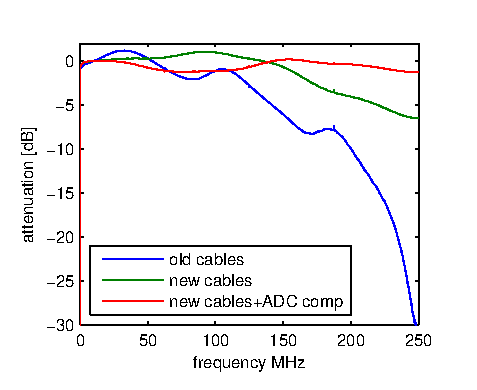
\includegraphics[width=\linewidth]{WEPD24_f2.eps}
\caption{Round trip attenuation of TMBF electronics (DAC connected to ADC) for different cables and ADC compensation filter.}
\label{cables}
\end{figure}

\section{Combined Tune Measurement and Bunch Cleaning}

 In operation we use a Numerically Controlled Oscillator (NCO) with a
programmable sweep function together with a numerical I/Q mixer and accumulator
for continuous measurement of the betatron tune oscillation frequency
\cite{status} with minimal disturbance to the beam by exciting only one bunch.

A new feature now allows to extend this beyond a simple sweep into a sequence of up to 7 `states', each of which can be a swept or fixed frequency (or no) excitation, and have the output of the I/Q mixers recorded or discarded.
In practice this has been used for `permanent bunch cleaning' of the fill pattern: Dark current from the LINAC gets accelerated through the booster and causes a low background of charge injected into a train of bunches before and after the actual `single bunch' that is used for filling and top-up injection. However, for some time resolved beamline experiments it is essential to keep a single bunch (in a hybrid or cam-shaft fill pattern) as clean as possible. To this end, we have implemented the following sequence of states:
\begin{enumerate}
\item Excite all `unwanted' bunches with full amplitude on the vertical plane while sweeping \textbf{backwards} over the betatron resonance frequency. Stabilise all other bunches using feedback. Discard I/Q data.
\item Excite one `designated' bunch with small amplitude to measure betatron tune frequency by recording I/Q data and finding peak. Stabilise all other bunches using feedback.
\item Stabilise all bunches using feedback until next sequence run is triggered.
\end{enumerate}

\begin{figure}%[!ht]
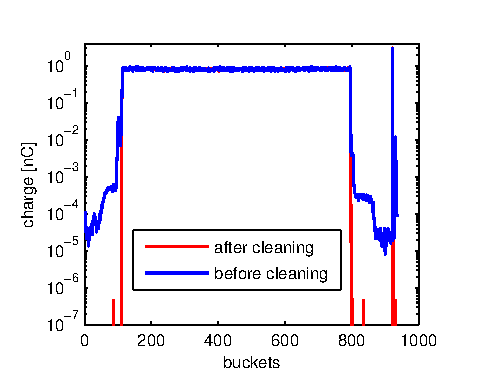
\includegraphics[width=\linewidth]{WEPD24_f1.eps}
\caption{Fill pattern before and after bunch cleaning.}
\label{cleaning}
\end{figure}

It should be emphasised that this process can take place permanently during user operation without any noticeable disturbance of the beam. To this end, it is important that DAC pre-emphasis  is used and the gain is switched from +1 to -1 before and after the single bunch so not to excite it \cite{capabilities}. In this way, even the regular injections into unwanted buckets during top-up operation can be cleaned away immediately.


\section{Fast Scanning of Transverse Mode Damping}
\begin{figure*}%[!ht]
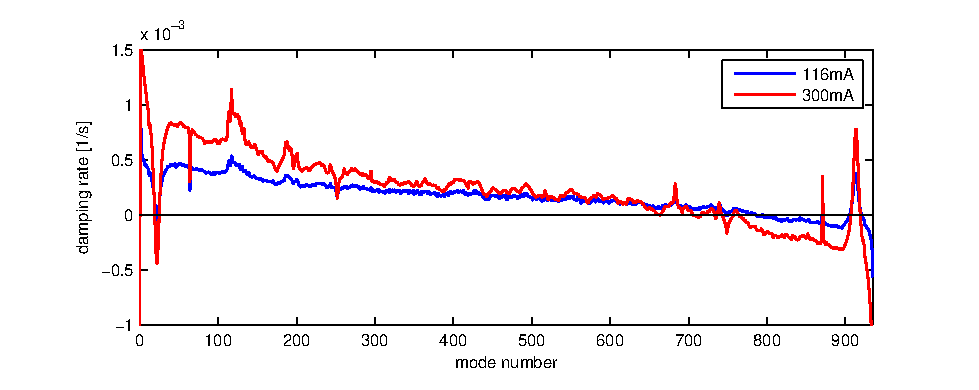
\includegraphics[width=\linewidth]{WEPD24_f3.eps}
\caption{Natural damping rates of all vertical modes as a function of beam current in a uniform fill pattern, with chromaticity set to 0}
\label{grow-damp}
\end{figure*}
In order to assess the damping (or growth) rates of individual transverse multi-bunch modes there are in principle two methods commonly referred to  \cite{teytelman,prabhakar}:
\begin{itemize}
\item The feedback is switched off for a short period (or even inverted to drive all modes), then the feedback is turned back on.  Bunch-by-bunch data is recorded from the point of switching off the feedback to some point after switching it back on to observe both growth and damping. This data is then transferred to an off-line analysis, which disseminates it mode by mode and analyses the individual growth rates. The limitation of this approach is that it will only show those modes which are unstable without active damping (or a few more if gain inversion is used). However, it is a very fast experiment which will require only a disturbance lasting typically a few ms.
\item An individual mode is excited using the NCO, this is followed by a period of a bunch-by-bunch recording during which after some delay the feedback is switched on again. Both the natural damping (or growth) and the active damping are recorded, however, only for one specific mode. This experiment then needs repeating for each mode. If bunch-by-bunch data is recorded the volumes of data created by the whole process can be quite large.
\end{itemize}
The second method has the ability to probe the damping times of each individual mode, no matter how close to instability it is. In the past, it would however been typically prohibitively slow to run through the repeated process of exciting, recording and data transferring for the typically high number of modes (there are 936 modes at DLS). We have significantly sped up this process (which is, at least with our current hardware, dominated by data transfer times) by two means:
\begin{itemize}
\item Instead of recording bunch-by-bunch data, we use the I/Q detector to determine the complex amplitude of the probed mode on a turn by turn basis. In our case, this reduces the amount of data to be stored and transferred for a typical scan of 936 modes of 750 turn grow-damp experiment from 1.3~GB to 5.6~MB.
\item Rather than performing one grow-damp experiment each and then transferring the data, we store all the I/Q data in the on board memory, and only read out once all modes have been scanned. The multi state sequencer has been extended to repeat with a programmable list of offset frequencies to this end. Thus a full scan of all 936 modes can be performed within 1.3s, plus a further 2s for data transfer and analysis.
\end{itemize}
The collected data is then analysed by assuming an exponential decay of the mode amplitude (that is the magnitude of the turn-by-turn I/Q data). A straight line fit to the logarithm of the magnitude is used to calculated the damping or growth rate, which is then plotted per mode. As these experiments can be repeated rapidly, it is now possible to scan parameters (like beam current, fill pattern, chromaticity) and see the effect on the damping rates in near real time.

Figure \ref{grow-damp} shows an example of the vertical damping rates as a function of beam current. It is clearly visible that more modes become unstable and the growth rates of the unstable modes (with negative damping rate) become larger (more negative). The overall slope across modes and the two distinct features at mode numbers 23 and 913 are understood from beam dynamics as a result of the resistive wall wake field. On the other hand, narrow features like at mode number 64 require further investigation, even if not currently leading to an instability, as these indicate narrow band resonators for instance as a result of long range wake fields.

\section{Fast Tune Following using PLL}
\begin{figure*}%[!ht]
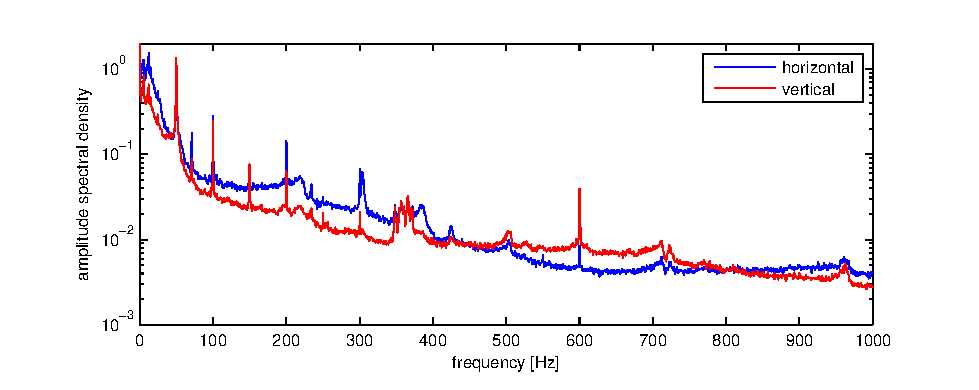
\includegraphics[width=\linewidth]{WEPD24_f4.eps}
\caption{Spectra computed from betatron tune frequency data recorded using the PLL}
\label{tunespectra}
\end{figure*}

Our normally used method of swept excitation and detection to determine the betatron tune frequency \cite{status} will typically measure the tune once per second. However, we have noticed that the betatron tunes exhibit continuous and fast small movements with a standard deviation of $\approx10^{-4}$ fractional tune units. These can be investigated in more detail using a tune following mechanism employing a PLL.

In this method, we continue to excite one or many bunches using the NCO, but rather than sweeping the NCO frequency, we detect the phase of the oscillating bunches relative to the excitation, low pass filter and feed it back through a proportional-integral controller to the NCO frequency. The number of turns observed to detect the phase is configurable, but in a typical setup we measure for 100~turns thus giving us a tune frequency reading every 187~$\mathrm{\mu s}$. The tune frequency readings are stored in a 4096 point buffer which can then be conveniently read out every time it updates to collect a long term record of tune stability at high update rate.

Figure \ref{tunespectra} shows the amplitude spectral density calculated from a 1 million point long record covering a total duration of 3 minutes. For this particular graph, the large number of points was split into 128 blocks which have been fourier transformed individually and then power averaged to produce spectra with precise amplitude densities rather than ultra fine frequency resolution. The spectra show that most of the movement of the betatron tunes is at low frequencies of a few 10~Hz, similar to orbit motion. There are also distinct lines at mains frequency and its harmonics.

The PLL tune measurement can also be used to measure the tune with higher precision by low pass filtering the stream of measurements, thus tracking the average tune value. This improves the uncertainty of tune measurements from $10^{-4}$ as achieved using the swept excitation (limited by tune motion during the sweep) to better than $10^{-5}$ at an update rate of once per second.

\section{Conclusions}
We presented some examples of the new types of measurements that have been enabled by a firmware development and upgrade of our existing TMBF system. The fundamental concept of the excitation using NCO and I/Q detection of bunch oscillations has been made more flexible by implementing complex sequences of excitations and PLL controlled tracking of the excitation. In particular, we expect the method of fast scanning of transverse mode damping times to be extensively used in probing transverse impedance of the storage ring and gathering a better understanding of the driving terms of instabilities.



\begin{thebibliography}{10}

\bibitem{libera}
Instrumentation Technologies, \emph{Libera Bunch-by-Bunch},
\url{http://www.i-tech.si}.

\bibitem{early-tmbf}
A.F.D.~Morgan, G.~Rehm, I.~Uzun, \emph{First Tests of the Transverse Multibunch
Feedback at Diamond}, DIPAC~2007

\bibitem{esrf}
E.~Plouviez, P.~Arnoux, F.~Epaud, J.~Jacob, J.M.~Koch, N.~Michel, G.A.~Naylor,
J.\mbox{-}L.~Revol, V.~Serriere, D.~Vial, \emph{Broadband Bunch by Bunch
Feedback for the ESRF using a Single High Resolution and Fast Sampling FPGA
DSP}, EPAC~2006.

\bibitem{performance}
A.F.D.~Morgan, G.~Rehm, I.~Uzun, \emph{Performance and Features of the Diamond
TMBF System}, EPAC~2008.

\bibitem{status}
I.~Uzun, M.G.~Abbott, M.T.~Heron, A.F.D.~Morgan, G.~Rehm, \emph{Operational
Status of the Transverse Multibunch Feedback System at Diamond}, ICALEPCS~2011.

\bibitem{measurement}
G.~Rehm, M.G.~Abbott, A.F.D.~Morgan, J.~Rowland, I.~Uzun, \emph{Measurement of
Lattice Parameters Without Visible Disturbance to User Beam at Diamond Light
Source}, BIW~2010.

\bibitem{capabilities}
M.G.~Abbott, G.~Rehm, I.~Uzun, \emph{Capability Upgrade of the Diamond Transverse Multibunch Feedback}, IBIC~2013.

\bibitem{capabilities2}
M.G.~Abbott, \emph{Extending the Capabilities of the Transverse Multibunch Feedback
Processor at Diamond}, Libera Workshop 2014, \newline {\scriptsize\url{http://www.i-tech.si/file/download/333_a8fc22df128d}}


\bibitem{teytelman}
D.~Teytelman, \emph{Architectures and Algorithms for Control and Diagnostics of
Coupled-Bunch Instabilities in Circular Accelerators}, PhD thesis, SLAC report 633.

\bibitem{prabhakar}
S.~Prabhakar, \emph{New Diagnostics and Cures for Coupled-Bunch Instabilities}, Phd thesis, SLAC report 554.
\end{thebibliography}
\vspace{0mm}

\end{document}
